\section{Turing Maschinen}
    
    
        \subsection{Motivation und Überblick}
        Formalisierung notwendig, um mathematisch über die automatische Unlösbarkeit zu argumentieren.
    
        Jede vernünftige Programmiersprache ist eine zulässige Formalisierung. 
    
        Aber nicht geeignet (meistens komplexe Operationen).
    
        Die Turingmaschine erlaubt ein paar \textbf{elementare Operationen} und besitzt trotzdem die \textbf{volle Berechnungsstärke} beliebiger Programmiersprachen.
    
        Ziel dieses Kapitels ist, dass ihr ein gewisse Gespür dafür bekommt, was eine Turingmaschine kann und was nicht.
    
    
    
        \subsection{Turing Maschinen - Formalisierung von Algorithmen}
        \begin{subbox}{Informell}
            Eine Turingmaschine besteht aus 
            \begin{enumerate}[label=(\roman*)]
                \item einer endlichen Kontrolle, die das Programm enthält,
                \item einem unendlichen Band, das als Eingabeband, aber auch als Speicher (Arbeitsband) zur Verfügung steht, und 
                \item einem Lese-/Schreibkopf, der sich in beiden Richtungen auf dem Band bewegen kann.
            \end{enumerate}
        \end{subbox}
        Für formale Beschreibung siehe Buch.
    
        \begin{figure}[htp]
            \centering
            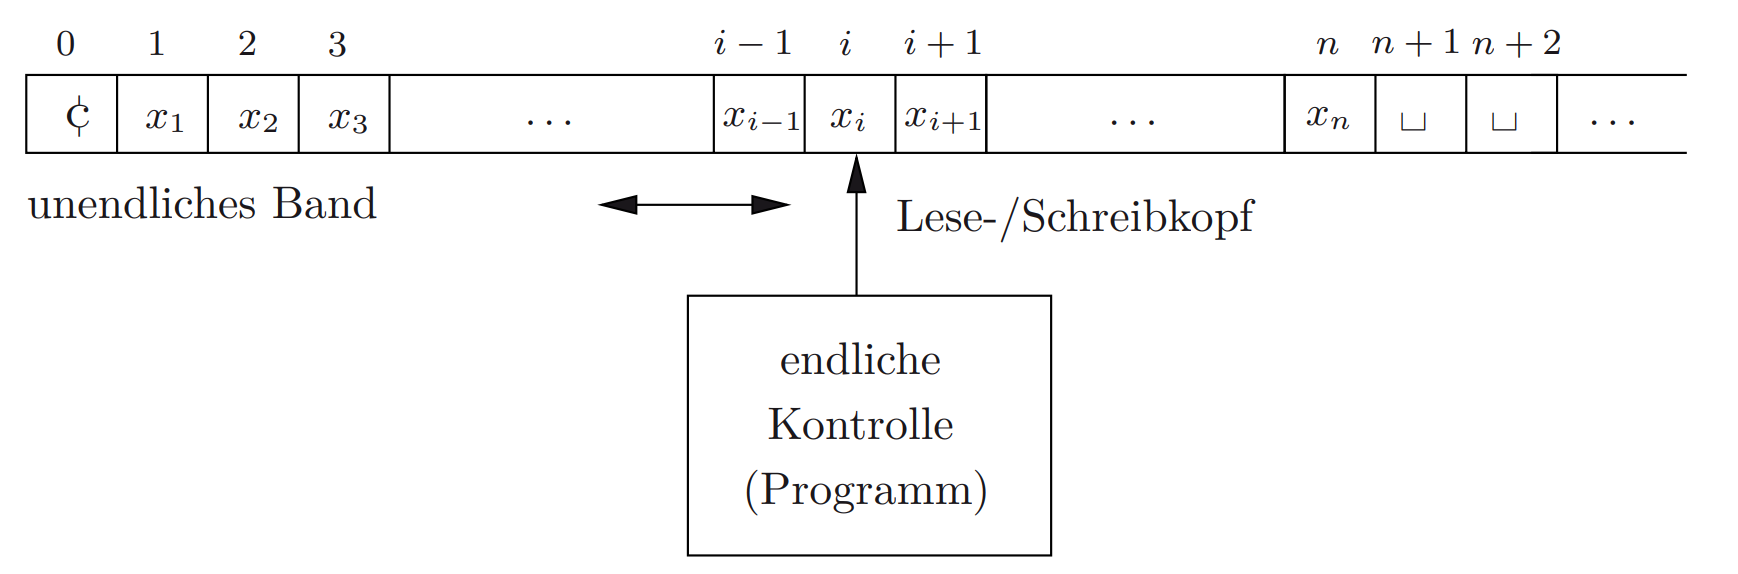
\includegraphics[width=0.7\textwidth]{Images/Turingmaschine.png}
            \caption{Abb. 4.1 vom Buch}
        \end{figure}
    
        \begin{mainbox}{Elementare Operation einer TM - Informell}
            \textbf{Input}
            \begin{itemize}[label = -]
                \item Zustand der Maschine (der Kontrolle)
                \item Symbol auf dem Feld unter dem Lese-/Schreibkopf
            \end{itemize}
            \textbf{Aktion}
            \begin{enumerate}[label=(\roman*)]
                \item ändert Zustand
                \item schreibt auf das Feld unter dem Lese-/Schreibkopf
                \item bewegt den Lese-/Schreibkopf nach links, rechts oder gar nicht. Ausser wenn $\cent$, dann ist links nicht möglich.
            \end{enumerate}
        \end{mainbox}
    
        \begin{mainbox}{}
            Eine \textbf{Konfiguration $C$} von $M$ ist ein Element aus 
            $$\textbf{Konf($\mathbf{M}$)} =  \{\cent\} \cdot \Gamma^* \cdot Q \cdot \Gamma^+ \cup Q \cdot \{\cent\} \cdot \Gamma^*$$
        \end{mainbox}
        \begin{itemize}[label=-]
            \item Eine Konfiguration $\cent w_1qaw_2$ mit $w_1, w_2 \in \Gamma^*$, $a \in \Gamma$ und $q \in Q$ sagt uns:
            
            $M$ im Zustand $q$, Inhalt des Bandes $\cent w_1aw_2 \text{\textvisiblespace} \text{\textvisiblespace} \text{\textvisiblespace}...$, Kopf an Position $|w_1|+1$ und liest gerade $a$.
            \item Eine Konfiguration $p\cent w$ mit $p \in Q$, $w\in \Gamma^*$: Inhalt des Bandes $\cent w \text{\textvisiblespace}  \text{\textvisiblespace}  \text{\textvisiblespace}...$, Zustand $p$ und Kopf an Position $0$. 
        \end{itemize}
        Bmk: Im Buch haben sie in der Definition von Konf $\Gamma^+$ anstatt $\Gamma^*$ an ''letzter Stelle''.
    
        Es gibt wieder eine Schrittrelation $\sststile{M}{} \subseteq \text{Konf}(M) \times \text{Konf}(M)$.
    
        \begin{figure}[htp]
            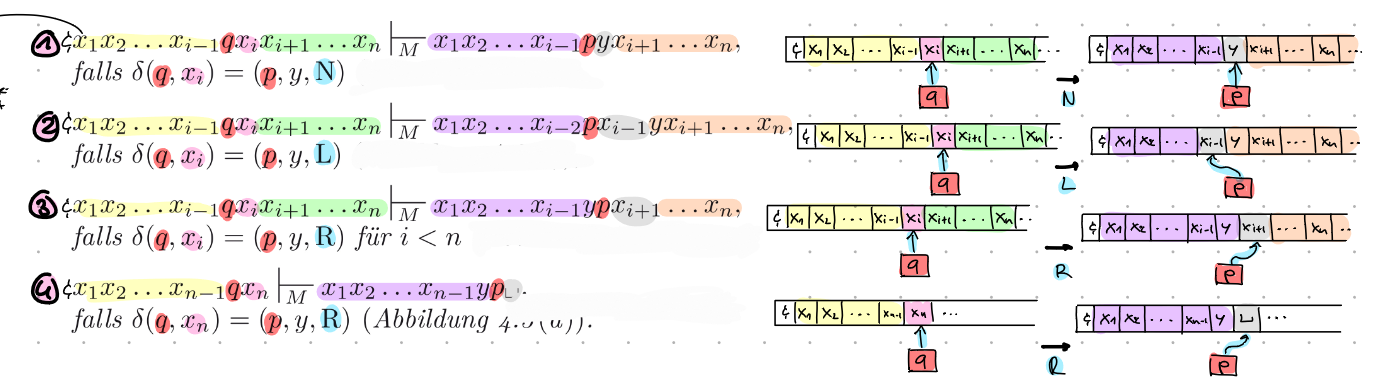
\includegraphics[width=\textwidth]{Images/Schrittrelation.png}
            \caption{Diagramm von Adeline}
        \end{figure}

        \comm{Zu beachten hier, ist dass bei einer Bewegung nach rechts, wobei der Kopf auf dem letzten Feld der Konfiguration war, das nächste 
        Feld zur Konfiguration hinzugefügt wird (4). In keiner Transition wird die Konfiguration verkürzt.}

    
        \textbf{Berechnung von $\mathbf{M}$}, \textbf{Berechnung von $\mathbf{M}$ auf einer Eingabe $\mathbf{x}$} etc. durch $\sststile{M}{}$ definiert.
    
        \begin{mainbox}{}
            Die Berechnung von $M$ auf $x$ heisst 
            \begin{itemize}[label=-]
                \item \textbf{akzeptierend}, falls sie in einer akzeptierenden Konfiguration $w_1q_{\text{accept}}w_2$ endet (wobei $\cent$ in $w_1$ enthalten ist).
                \item \textbf{verwerfend}, wenn sie in in einer verwerfenden Konfiguration $w_1q_{\text{reject}}w_2$ endet.
                \item \textbf{nicht-akzeptierend}, wenn sie entweder eine \textbf{verwerfende} oder unendliche Berechnung ist.
            \end{itemize}
        \end{mainbox}
    
        \begin{mainbox}{}
            Die von der \textbf{Turingmaschine $\mathbf{M}$ akzeptierte Sprache} ist 
            $$\mathbf{L(M)} = \{w \in \Sigma^* \mid q_0\cent w \sststile{M}{*}yq_{\text{accept}}z, \text{ für irgendwelche }y, z \in \Gamma^*\}$$
        \end{mainbox}
    
    
    
        \subsection{Wichtige Klassen}
        \begin{subbox}{Reguläre Sprachen}
            $$\mathbf{\mathcal{L}_{\textbf{EA}}} = \{L(A) \mid A \text{ ist ein EA}\} = {\mathcal{L}_{\textbf{NEA}}}$$
        \end{subbox}
    
        \begin{mainbox}{Rekursiv aufzählbare Sprachen}
            Eien Sprache $L \subseteq \Sigma^*$ heisst \textbf{rekursiv aufzählbar}, falls eine TM $M$ existiert, so dass $L = L(M)$.
            $$\mathbf{\mathcal{L}_{\textbf{RE}}} = \{L(M) \mid M \text{ ist eine TM}\}$$
            ist die \textbf{Klasse aller rekursiv aufzählbaren Sprachen}.
        \end{mainbox}
    
        \begin{subbox}{Halten}
            Wir sagen das $M$ \textbf{immer hält}, wenn für alle Eingaben $x \in \Sigma^*$
            \begin{enumerate}[label=(\roman*)]
                \item $q_0\cent x \sststile{M}{*} yq_{\text{accept}}z, y,z \in \Gamma^*, \text{ falls }x \in L \text{ und }$
                \item $q_0 \cent x \sststile{M}{*} uq_{\text{reject}}v, u,v \in \Gamma^*, \text{ falls }x \notin L.$
            \end{enumerate}
        \end{subbox}
    
        \begin{mainbox}{Rekusive Sprachen}
            Eine Sprache $L \subseteq \Sigma^*$ heisst \textbf{rekursiv (entscheidbar)}, falls $L = L(M)$ für eine TM $M$, die \textbf{immer hält}.
            $$\mathbf{\mathcal{L}_{\textbf{R}}} = \{L(M) \mid M \text{ ist eine TM, die immer hält}\}$$
            ist die \textbf{Klasse der rekursiven (algorithmisch erkennbaren) Sprachen}.
        \end{mainbox}
    
    
    
        \subsection{Mehrband-Turingmaschine}
        \begin{mainbox}{Mehrband-TM - Informelle Beschreibung}
            Für $k \in \N\setminus\{0\}$ hat eine $k$-Band Turingmaschine 
            \begin{itemize}[label=-]
                \item eine endliche Kontrolle 
                \item ein endliches Band mit einem Lesekopf (Eingabeband)
                \item $k$ Arbeitsbänder, jedes mit eigenem Lese-/Schreibkopf (nach rechts unendlich)
            \end{itemize}
        \end{mainbox}
        \textbf{Insbesondere gilt $1$-Band TM $\neq$ ''normale'' TM}
    
        Am Anfang der Berechnung einer MTM $M$ auf $w$
        \begin{itemize}[label=-]
            \item Arbeitsbänder ''leer'' und die $k$ Lese-/Schreibköpfe auf Position $0$.
            \item Inhalt des Eingabebands $\cent w \$$ und Lesekopf auf Position $0$.
            \item Endliche Kontrolle im Zustand $q_0$.
        \end{itemize}
    
    
    
        \subsection{Äquivalenz von Maschinen (TM, MTM)}
        \begin{mainbox}{}
            Seien $A$ und $B$ zwei Maschinen mit \textbf{gleichem} $\Sigma$.
    
            Wir sagen, dass \textbf{$\mathbf{A}$ äquivalent zu $\mathbf{B}$ ist}, wenn für jede Eingabe $x \in \Sigma^*$
            \begin{enumerate}[label=(\roman*)]
                \item $A$ akzeptiert $x$ $\iff$ $B$ akzeptiert $x$
                \item $A$ verwirft $x$ $\iff$ $B$ verwirft $x$
                \item $A$ arbeitet unendlich lange auf $x$ $\iff$ $B$ arbeitet unendlich lange auf $x$
            \end{enumerate}
        \end{mainbox}
        Wir haben 
        \begin{center}
            $A$ und $B$ äquivalent $\implies$ $L(A) = L(B)$
    
            aber 
    
            $L(A) = L(B)$ $\centernot{\implies}$ $A$ und $B$ äquivalent
        \end{center}
        da $A$ auf $x$ unendlich lange arbeiten könnte, während $B$ $x$ verwirft.
    
        \begin{mainbox}{Lemma 4.1}
            Zu jeder TM $A$ existiert eine zu $A$ äquivalente 1-Band-TM $B$
        \end{mainbox}
        \textbf{Beweisidee}
        $B$ kopiert die Eingabe zuerst aufs Arbeitsband und simuliert dann $A$.
    
        \begin{mainbox}{Lemma 4.2}
            Zu jeder Mehrband-TM $A$ existiert eine zu $A$ äquivalente TM $B$
        \end{mainbox}
        \textbf{Beweis}
        
        Sei $A$ eine $k$-Band-Turingmaschine für ein $k \in \N \setminus \{0\}$. Wir konstruieren eine TM $B$, die Schritt für Schritt $A$ simuliert.

        $B$ speichert die Inhalte aller $k+1$ Bänder von $A$ auf ihrem einzigen Band. Anschaulich gesprochen ist jedes Feld auf dem Band von $B$ ein $2(k+1)$-Tupel und jedes Element dieses Tupels ist auf einer Spur. 
        Sei $\Gamma_A$ das Arbeitsalphabet von $A$. Dann gilt 
        $$\Gamma_B = (\Sigma_A \cup \{\cent, \$, \text{\textvisiblespace}\}) \times \{\text{\textvisiblespace},\uparrow\} \times (\Gamma_A \times \{\text{\textvisiblespace}, \uparrow\})^k \cup \Sigma_A \cup \{\text{\textvisiblespace}, \cent\}$$
        Für ein Symbol $\alpha = (a_0,a_1,a_2,...,a_{2k+1}) \in \Gamma_B$ sagen wir, dass $a_i$ auf der $i$-ten Spur liegt. Daher bestimmen die $i$-ten Elemente der Symbole auf dem Band von $B$ den Inhalt der $i$-ten Spur. Eine Konfiguration $(q,w,i,x_1,i_1,x_2,i_2,...,x_k,i_k)$ von $A$ ist dann in $B$ wie folgt gespeichert. 
        \begin{itemize}
            \item Der Zustand $q$ ist in der endlichen Kontrolle von $B$ gespeichert. 
            \item Die $0$-te Spur des Bandes von $B$ enthält die $\cent w\$$ (i.e. den Inhalt des Eingabebandes von $A$)
            \item Für alle $i \in \{1, ..., k\}$ enthält die $(2i)$-te Spur des Bandes von $B$ den Inhalt vom $i$-ten Band von $A$ (i.e. $\cent x_i\$$).
            \item Für alle $i \in \{1, ..., k\}$ bestimmt die $(2i +1)$-te Spur des Bandes von $B$ mit dem Symbol $\uparrow$ die Position des Kopfes auf dem $i$-ten Arbeitsband von $A$.
        \end{itemize}
        Ein Schritt von $A$ kann jetzt durch folgende Prozedur von $B$ simuliert werden:
        \begin{enumerate}
            \item $B$ liest einmal den Inhalt ihres Bandes von links nach rechts, bis sie alle $k+1$ Kopfpositionen von $A$ gefunden hat, und speichert dabei in ihrem Zustand die $k+1$ Symbole, die an diesen Positionen stehen. (Dies kann ohne weiteres in der Zustandsmenge abgespeichert werden, da $k$ fix ist, folglich ist dann $\Gamma_A^k$ auch endlich)
            \item Nach der ersten Phase kennt $B$ das ganze Argument (der Zustand von $A$ ist im Zustand von $B$ gespeichert) der Transitionsfunktion von $A$ und kann also die entsprechenden Aktionen (Köpfe bewegen, Ersetzen von Symbolen) von $A$ bestimmen. Diese Änderungen führt $B$ in einem Lauf über ihr Band von rechts nach links durch.
        \end{enumerate}
        \hspace*{0pt}\hfill$\blacksquare$
    
        Aus Lemma 4.1 und 4.2 folgt direkt
        \begin{mainbox}{Satz 4.1}
            Die Maschinenmodelle von Turingmaschinen und Mehrband-Turingmaschinen sind äquivalent.
        \end{mainbox}
        Note: 
        \begin{itemize}
            \item ''Äquivalenz'' für Maschinenmodelle wird in Definition 4.2 definiert.
            \item Maschinenmodelle sind Klassen von Maschinen (i.e. Mengen von Maschinen mit gewissen Eigenschaften).
        \end{itemize}
    
        \subsection{Nichtdeterministische Turingmaschinen}
            \begin{mainbox}{Definition von NTM}
                Eine \textbf{nichtdeterministische Turingmaschine (NTM)} ist ein $7$-Tupel $M = (Q, \Sigma, \Gamma, \delta, q_0, q_{\text{accept}}, q_{\text{reject}})$, wobei 
                \begin{enumerate}[label=(\roman*)]
                    \item $Q, \Sigma, \Gamma, q_{\text{accept}}, q_{\text{reject}}$ die gleiche Bedeutung wie bei einer TM haben, und
                    \item $\delta: (Q \setminus \{q_{\text{accept}}, q_{\text{reject}}\}) \times \Gamma \to \mathcal{P}(Q \times \Gamma \times \{\text{L, R, N}\})$ 
                    die \textbf{Übergangsfunktion} von $M$ ist und die folgende Eigenschaft hat:
                    $$\delta(p, \cent) \subseteq \{(q, \cent, X) \mid q \in Q, X \in \{R, N\}\}$$
                    für alle $p \in Q$
                \end{enumerate}
            \end{mainbox}
            \textbf{Konfiguration} ähnlich wie bei TMs.
            \begin{center}
                Konfiguration akzeptierend $\iff$ enthält $q_{\text{accept}}$\\
                Konfiguration verwerfend $\iff$ enthält $q_{\text{reject}}$
            \end{center}
        
        
        
            \textbf{Die üblichen Sachen}
            \begin{itemize}[label=-]
                \item Schrittrelation $\sststile{M}{}$ ''verbindet zwei Konfigurationen, wenn man von der einen in die andere kommen kann''
                \item Reflexive und transitive Hülle ist $\sststile{M}{*}$.
                \item Berechnung von $M$ ist eine Folge von Konfigurationen $C_1, C_2, ...$, so dass $C_i \sststile{M}{} C_{i+1}$.
                \item Eine Berechnung von $M$ auf $x$ ist beginnt in $q_0\cent x$ und endet entweder unendlich oder endet in $\{q_{\text{accept}}, q_{\text{reject}}\}$.
            \end{itemize}
            \begin{mainbox}{Akzeptierte Sprache}
                $$L(M) = \{w \in \Sigma^* \mid q_0\cent w \sststile{M}{*} yq_{\text{accept}}z \text{ für irgendwelche }y,z \in \Gamma^*\}$$
            \end{mainbox}
        
        
        
            \textbf{Berechnungsbaum}
            \begin{mainbox}{}
                Sei $M=  (Q, \Sigma, \Gamma, \delta, q_0, q_{\text{accept}}, q_{\text{reject}})$ eine NTM 
                und sei $x$ ein Wort über dem Eingabealphabet $\Sigma$ von $M$. 
                Ein \textbf{Berechnungsbaum $\mathbf{T_{M, x}}$ von $\mathbf{M}$ auf $\mathbf{x}$} ist ein 
                (potentiell unendlicher) gerichteter Baum mit einer Wurzel, der wie folgt definiert wird.
        
                \begin{enumerate}[label=(\roman*)]
                    \item Jeder Knoten von $T_{M,x}$ ist mit einer Konfiguration beschriftet.
                    \item Die Wurzel ist der einzige Knoten von $T_{M,x}$ mit dem Eingangsgrad $0$ und ist mit der Startkonfiguration $q_0\cent x$ beschriftet.
                    \item Jeder Knoten des Baumes, der mit einer Konfiguration $C$ beschriftet ist, hat genauso viele Kinder wie $C$ Nachfolgekonfigurationen hat, und diese Kinder sind mit diesen Nachfolgekonfigurationen $C$ markiert.
                \end{enumerate}
            \end{mainbox}
        
        
        
            \textbf{Äquivalenz NTM und TM}
            \begin{mainbox}{Satz 4.2}
                Sei $M$ eine NTM. Dann existiert eine TM $A$, so dass 
                \begin{enumerate}[label=(\roman*)]
                    \item $L(M) = L(A)$ und 
                    \item falls $M$ keine unendlichen Berechnungen auf Wörtern aus $L(M)^\complement$ hat, dann hält $A$ immer.
                \end{enumerate}
            \end{mainbox}
            \textbf{Beweisidee:} 
            
            ''BFS im Berechnungsbaum'', i.e. wir simulieren einzelne Schritte der verschiedenen Berechnungsstränge mit 
            zwei Bändern, wobei das erste Band alle Konfigurationen der besuchten Schicht speichert und das zweite 
            alle Konfigurationen der nächsten Schicht.

            Wenn eine akzeptierende Konfiguration erreicht wird, dann akzeptiert $A$. 
            Wenn keine weitere Konfiguration erreichbar ist, dann verwirft $A$ (eine verwerfende Konfiguration wird ohne weiteres normal behandelt). 
        
        